\documentclass[12pt]{article}
\usepackage[top=1in, bottom=1in, left=1in, right=1in]{geometry}

\usepackage{setspace}
\onehalfspacing

\usepackage{amssymb}
%% The amsthm package provides extended theorem environments
\usepackage{amsthm}
\usepackage{epsfig}
\usepackage{times}
\renewcommand{\ttdefault}{cmtt}
\usepackage{amsmath}
\usepackage{graphicx} % for graphics files
\usepackage{tabu}

% Draw figures yourself
\usepackage{tikz} 

% writing elements
\usepackage{mhchem}

% The float package HAS to load before hyperref
\usepackage{float} % for psuedocode formatting
\usepackage{xspace}

% from Denovo Methods Manual
\usepackage{mathrsfs}
\usepackage[mathcal]{euscript}
\usepackage{color}
\usepackage{array}

\usepackage[pdftex]{hyperref}
\usepackage[parfill]{parskip}

% math syntax
\newcommand{\nth}{n\ensuremath{^{\text{th}}} }
\newcommand{\ve}[1]{\ensuremath{\mathbf{#1}}}
\newcommand{\Macro}{\ensuremath{\Sigma}}
\newcommand{\rvec}{\ensuremath{\vec{r}}}
\newcommand{\vecr}{\ensuremath{\vec{r}}}
\newcommand{\omvec}{\ensuremath{\hat{\Omega}}}
\newcommand{\vOmega}{\ensuremath{\hat{\Omega}}}
\newcommand{\sigs}{\ensuremath{\Sigma_s(\rvec,E'\rightarrow E,\omvec'\rightarrow\omvec)}}
\newcommand{\el}{\ensuremath{\ell}}
\newcommand{\sigso}{\ensuremath{\Sigma_{s,0}}}
\newcommand{\sigsi}{\ensuremath{\Sigma_{s,1}}}
%---------------------------------------------------------------------------
%---------------------------------------------------------------------------
\begin{document}
\begin{center}
{\bf NE 155/255, Fall 2019\\
November 20, 2019 \\
CADIS and FW-CADIS
}
\end{center}

\textbf{Making an Importance/Weight Map}\\
How do we assign importances to a problem? We can do it by hand. E.g.\ you can
assign each geometry component an importance based on what you think should be
happening. All splitting and rouletting is based on the importance ratios
between geometric cells. Guidance to do this is to keep adjacent cells within a
factor of a few of one another and to keep cells only about two mean free paths
thick. It is one thing to think about doing that in a 1D slab (and it still may
be too hard to do\textemdash think about doing that accurately for a
six-order-of-magnitude fall off over 30 cm of lead), but choosing these
properly in 3D? Not so easy...

We would prefer to have an automated method that does not rely on guessing. The
Consistent Adjoint Driven Importance Sampling (CADIS) and Forward Weighted
(FW)-CADIS methods do just that. They were developed by John Wagner, Ali
Haghighat, and Douglas Peplow at Penn State and ORNL. We'll go through these
methods, highlighting conceptual ideas. In particular, we note the application of the adjoint.   

The forward flux describes the particle distribution as a result of system conditions. \\
The \textit{adjoint} flux describes how important the particle distribution is to the answer in question:
\begin{gather*}
-\omvec\cdot  \nabla \psi^{\dagger}(\rvec,E,\omvec) +
\Sigma_t(\rvec,E)\psi^{\dagger}(\rvec,E,\omvec) = \\
\int_0^{\infty}\int_{4\pi}
\Sigma_s(\rvec, E\rightarrow E',\omvec\rightarrow\omvec')
\psi^{\dagger}(\rvec,E',\omvec')d\omvec'dE'+Q^{\dagger}(\rvec, E, \omvec).
\end{gather*}

Note the differences -- the streaming term is negative on the left hand side of
the equation and the scattering term has particles going ``backwards'' in energy
and angle. We can think of this as asking: how did the particles get from where
they started to our response of interest?

The solution to the adjoint equation can be interpreted physically as particle
importance. If the adjoint flux in a region is high, then particles there are
likely to contribute to our forward response of interest, and we can say that
that region is important. On the other hand, if the adjoint flux is low in a
given region, it is unlikely that particles in that region will reach the
detector in the forward problem, so we can say that that phase space region is
less important.

Consider the plots in Figure \ref{fwd-adj} below.

\begin{figure}[!htb]
\centering
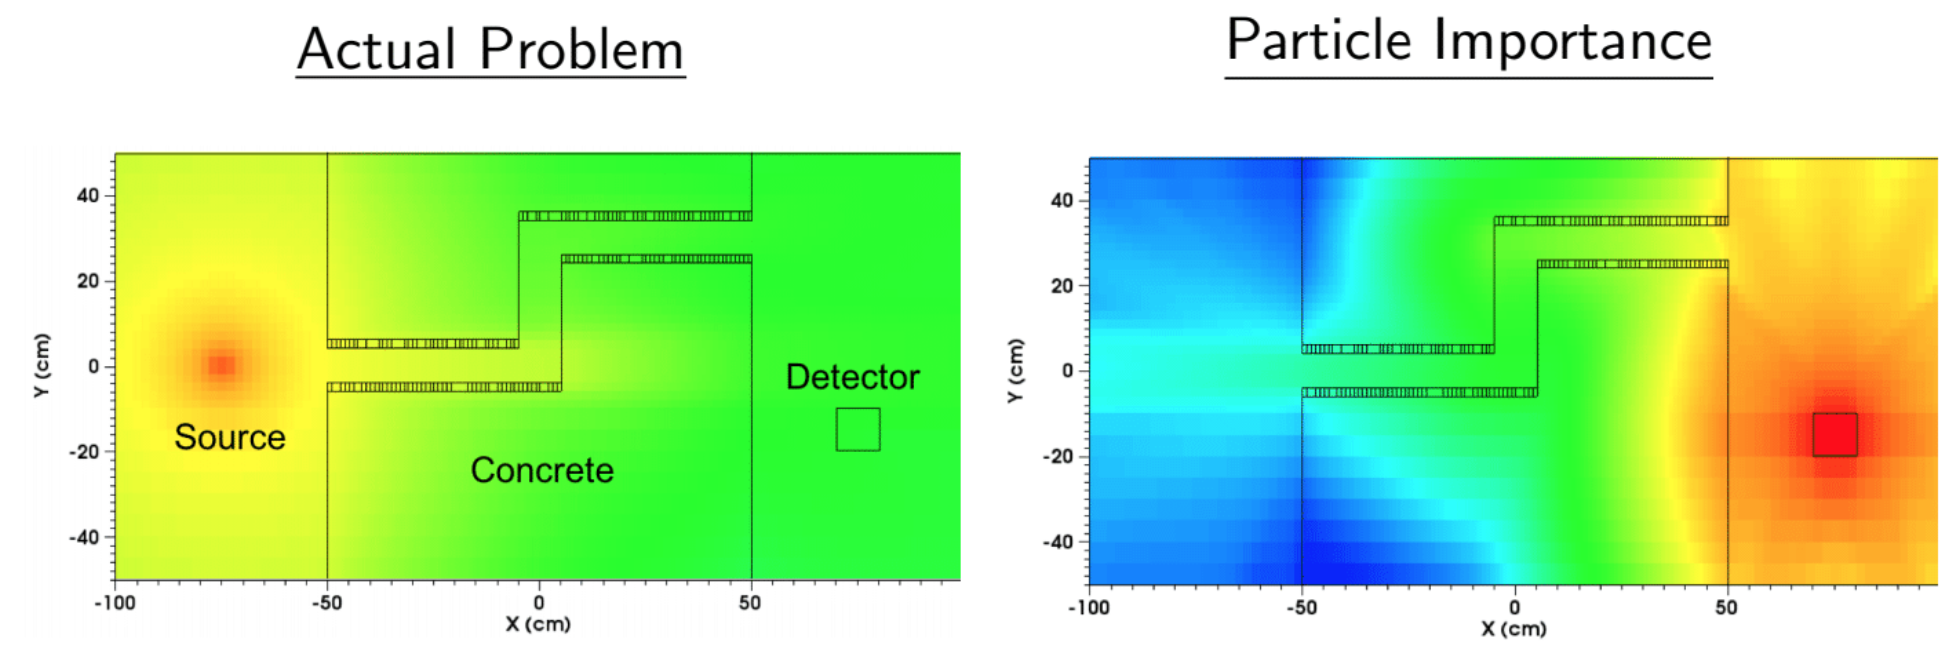
\includegraphics[width=\textwidth]{fig/fwd-adj.png}
\caption{Forward and adjoint scalar flux solution plots.}
\label{fwd-adj}
\end{figure}

The left plot is the ``forward solution''; particles start at the source and
we're interested in the response at the detector. The right plot is the
``adjoint solution''; we set the adjoint source to be the detector and then
interpret the resultant adjoint scalar flux solution as our importance map.
So, looking at the plot, we see that the bottom left corner of the concrete
shield is not a very important region of our phase space; it's unlikely that
a particle there will ever reach the detector in the forward problem.

It can be shown that some response of interest $R$ can be calculated as
\begin{align*}
R &= \int dV \int dE\: f(\vec{r}, E) \phi(\vec{r}, E) \quad \text{and}\\
&= \int dV \int dE\: \phi^{\dagger}(\vec{r}, E) q(\vec{r}, E)
\end{align*}
where $f$ is the response function of interest and angle is neglected for
simplicity. This is done by setting $Q^{\dagger} = f$ and using the adjoint
identity.

The physical interpretation of the adjoint flux is the influence or importance
of a particle in phase space to what we used for the adjoint source: it maps
source particles directly into the response.
Thus, if we set the response that we are solving for to be the adjoint source,
the adjoint flux is the importance map corresponding to that response. 

\textbf{CADIS}\\
These notes are derived from the SCALE manual descriptions. 

Note that if we had an accurate representation of $\phi^{\dagger}$, we would
then just have the answer. Solving for $\phi^{\dagger}$ is just as hard as
solving for $\phi$. The idea motivating CADIS is to use an approximate version
of $\phi^{\dagger}$ that was obtained quickly with a deterministic solver to
create VR parameters for MC. 

We use the adjoint flux to bias the source distribution, set target weights,
and choose particle birth weights:
\begin{align*}
\hat{Q}(\vec{r}, E) &= \frac{1}{R} Q(\vec{r}, E)\phi^{\dagger}(\vec{r}, E) \\
w_{nom} &= \frac{R}{\phi^{\dagger}(\vec{r}, E)}\\
w_0 &\equiv \frac{Q(\vec{r}, E)}{\hat{Q}(\vec{r}, E)} = \frac{R}{\phi^{\dagger}(\vec{r}, E)}\:,
\end{align*}
%
where $w_0$ is birth weight. Note that we need to set the birth weight this way
such that a fair game is preserved given the biased source sampling.

Further, notice that the birth weight exactly matches the target weight. This
means that computational time is not wasted splitting/rouletting particles 
immediately upon birth. The \textit{consistency} among these items is also the
source of the method's name.

\textbf{Multiple Tallies}\\
What if we want multiple tallies? For these problems, the user must accept a
total simulation time that is controlled by the tally with the slowest
convergence and simulation results where the tallies have a wide range of
relative uncertainties.

The obvious way around this problem is to create a separate problem for each
tally and use CADIS to optimize each. Each simulation can then be run until the
tally reaches the level of acceptable uncertainty. For more than a few tallies,
this approach becomes complicated and time-consuming for the user. For mesh tallies,
this approach is not reasonable.

Another approach to treat several tallies, if they are in close proximity to
each other, or a mesh tally covering a small portion of the physical problem,
is to use the CADIS methodology with the adjoint source near the middle of the
tallies to be optimized. Since particles in the forward Monte Carlo simulation
are optimized to reach the location of the adjoint source, all the tallies
surrounding that adjoint source should converge quickly.

The drawback to this approach is the difficult question of ``how close". If the
tallies are too far apart, certain energies or regions that are needed for one
tally may be of low importance for getting particles to the central adjoint
source. This may under-predict the flux or dose at some of the tally sites.

For several tallies that are far from each other, multiple adjoint sources
could be used. In the forward Monte Carlo, particles would be drawn to one of
those adjoint sources. The difficulty with this approach is that typically the
tally that is closest to the true physical source will converge faster than the
other tallies. Finding the correct relative source strengths so that all of the
tallies converged to the same relative uncertainty in one simulation then
becomes an iterative process for the user.

\textbf{FW-CADIS}\\
If we want the answer everywhere or in many locations (like in shielding or
some reactor and security calculations), we need a different approach: forward
weighting. There are two ways to think about why this works:

\textbf{1.} In order to converge several tallies to the same relative uncertainty in the
one simulation, the adjoint source corresponding to each of those tallies needs
to be weighted inversely by the expected tally value.

With mesh tallies, instead of using a uniform adjoint source strength over the
entire mesh tally volume, each voxel of the adjoint source should be weighted
inversely by the expected forward tally value for that voxel. Areas of low flux
or low dose rate would have more adjoint source strength than areas of high flux or high dose rate.

First, a forward, coarse deterministic calculation is done to estimate the
expected tally results.
A total adjoint source is constructed, where the adjoint source corresponding
to each tally is weighted inversely by those forward tally estimates.

\textbf{2.} (from Wagner) To get uniformly-low statistical uncertainty, it has
been proposed that the distribution of MC particles should be uniform throughout the system.
Although this is not a `physical' response, it does intuitively represent a
desirable objective for obtaining uniform uncertainty.
Using adjoint transport theory, we can define the adjoint source such that the
result is an importance function targeting uniform particle distribution.

\vspace*{1 em}
Either way you want to think about it, we do the same thing. 
We do a coarse deterministic calculation to get the forward flux and use it in constructing the adjoint source:
\begin{align*}
\text{Energy- and space-dependent flux, } \phi(\vec{r},E): \quad & Q^{\dagger}(\vec{r},E) = \frac{1}{\phi(\vec{r},E)}\\
\text{Space-dependent total flux, } \int dE\:\phi(\vec{r},E): \quad & Q^{\dagger}(\vec{r},E) = \frac{1}{\int dE\:\phi(\vec{r},E)}\\
\text{Space-dependent total dose rate, } \int dE\:\phi(\vec{r},E) \Sigma_d(\vec{r},E): \quad & Q^{\dagger}(\vec{r},E) = \frac{\Sigma_d(\vec{r},E)}{\int dE\:\phi(\vec{r},E)\Sigma_d(\vec{r},E)}
\end{align*} 
You can see the inverse weighting discussed in explanation (1), or you can think of how this impacts the approximate response (in this case defined as $\langle \phi, Q^{\dagger}\rangle$) for explanation (2):
\[
R(\vec{r},E) = \int dV \int dE \: \phi(\vec{r},E) \frac{1}{\phi(\vec{r},E)} \approx 1\:,
\]
where the approximately equals is because the $\phi$ values are rough guesses and can come from different calculations.

Again, if we had the global solution, wouldn't we be finished? The key to
FW-CADIS is to remember that both the forward and adjoint calculations are
coarse and hence very fast. It therefore takes a small amount of time to
create a very effective set of values used for source biasing, birth weight
setting, and weight window creation - where the weight windows are used for
splitting and rouletting. 

%-------------------------------------------------------

\end{document}